\chapter{Sistema Proposto}\label{cap3}

Essa seção apresenta as etapas de desenvolvimento do sistema de recuperação de atas proposto, bem como o seu funcionamento geral, desde a preparação dos documentos até a entrega dos históricos de ocorrência ao usuário. Inicialmente serão descritos a seleção e pré-processamento das atas. Em seguida, ... 


O sistema proposto tem como objetivo permitir ao usuário consultar uma coleção de documentos de reuniões a fim de obter todo o histórico de ocorrências de um determinado tema relacionado à pesquisa do usuário, podendo identificar nos documentos onde esse tema foi mencionado, bem como se houve uma decisão sobre o tema. Para isso, o sistema é divido em dois módulos principais: módulo de preparação e manutenção e módulo de consulta, os quais serão detalhados nas próximas seções.  % "isso envolve a classificação. Onde entram os tópicos?" --> Rafael


  %--- Figura Visão Geral ---
  \begin{figure}[!h]
	  \centering
	  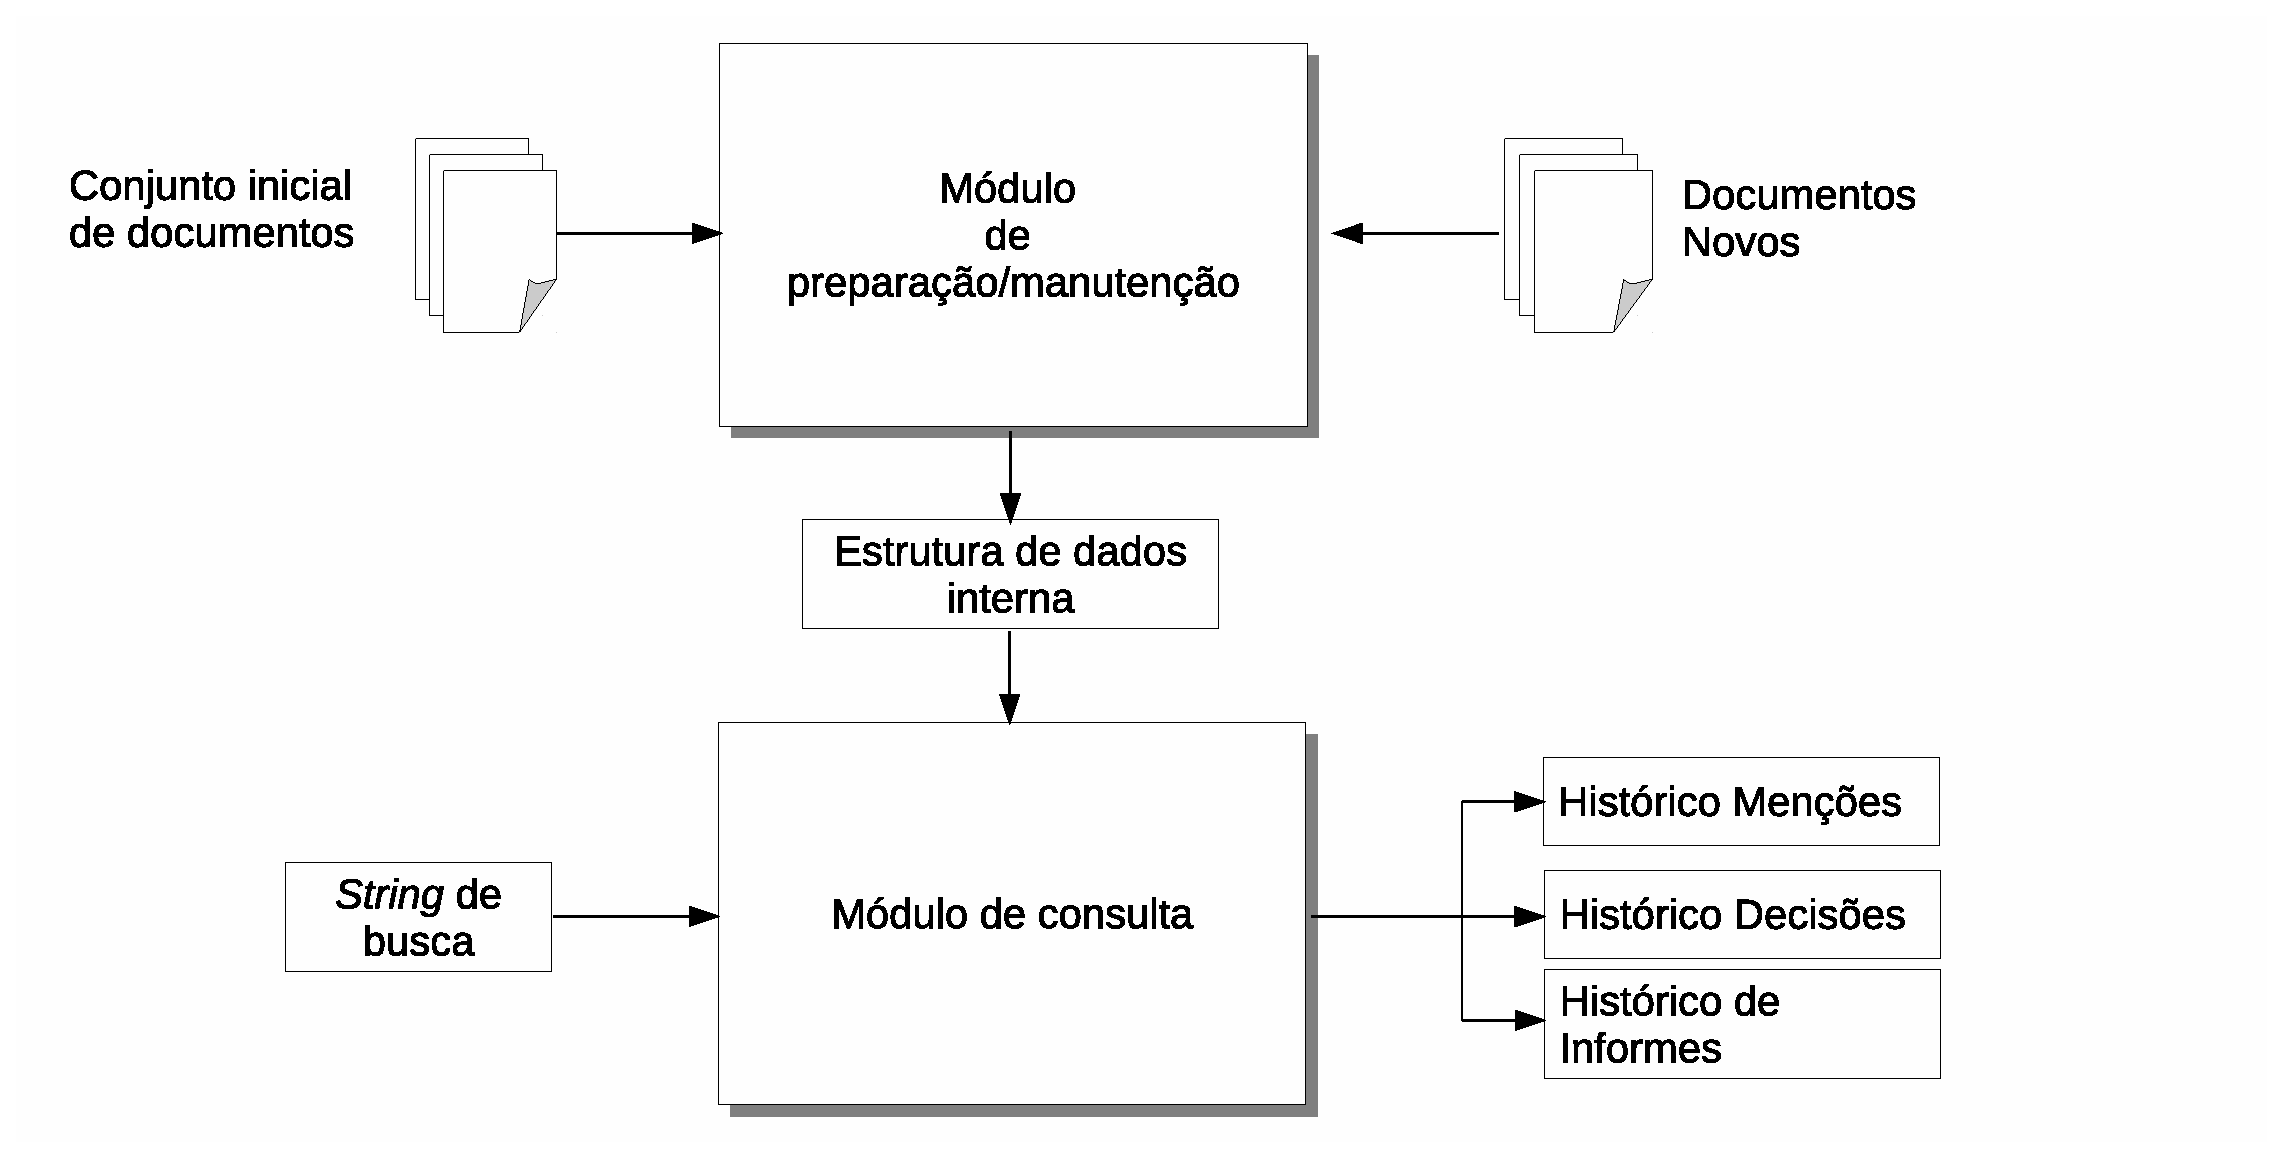
\includegraphics[width=0.69\paperwidth]{conteudo/capitulos/figs/visao-geral-3.eps}
	  \caption{Visão geral do sistema}
	  \label{fig:visao-geral}
  \end{figure}

A Figura \ref{fig:visao-geral} mostra a visão geral do sistema com suas principais entradas e saídas. Inicialmente o sistema recebe um conjunto inicial de documentos. A função de Módulo de preparação/manutenção é processar esses texto e gerar uma base de dados interna que codifica os textos extraídos com seus respetivos tópicos. O Módulo de consulta recebe a consulta do usuário que expressa o assunto de interesse. Em seguida, os trechos de texto que fazem menção ao esse assunto são exibidos ao usuário.


\section{Módulo de preparação e manutenção}\label{sec:modulo-preparacao}

O módulo de preparação e manutenção tem como funções principais dividir cada ata em em segmentos de texto que contêm um assunto predominante, e separá-los em categorias por meio de técnicas de extração tópicos e classificação. Além disso, produz uma estrutura de dados que registra quais assuntos foram tratados na reunião, bem como o trecho do documento onde é discutido.  

% melhorar ↓↓↓↓↓
% A seguir são apresentadas as etapas do módulo de preparação e manutenção desde a preparação dos documentos até a entrega da estrutura interna ao módulo de consulta. 


% ========== Preparação dos Documentos ==========


% \subsection{Preparação dos documentos}

As atas são normalmente armazenadas em arquivos binários do tipo \textit{pdf}, \textit{doc}, \textit{docx} ou \textit{odt}. As atas devem ser pré-processadas e estruturadas para que possam ser aplicados métodos de MI e RI. Inicialmente, o texto puro é extraído e passa por processos de transformação que incluem o pré-processamento do texto, remoção de elementos considerados menos significativos e a identificação de sentenças. Esse processo é ilustrado na Figura~\ref{fig:preprocessamento-segmentacao} e descrito a seguir.

	
% -<? Colocar aqui uma explicação do que é um segmento e uma sentença?

\begin{center}
	\begin{figure}[h!]

	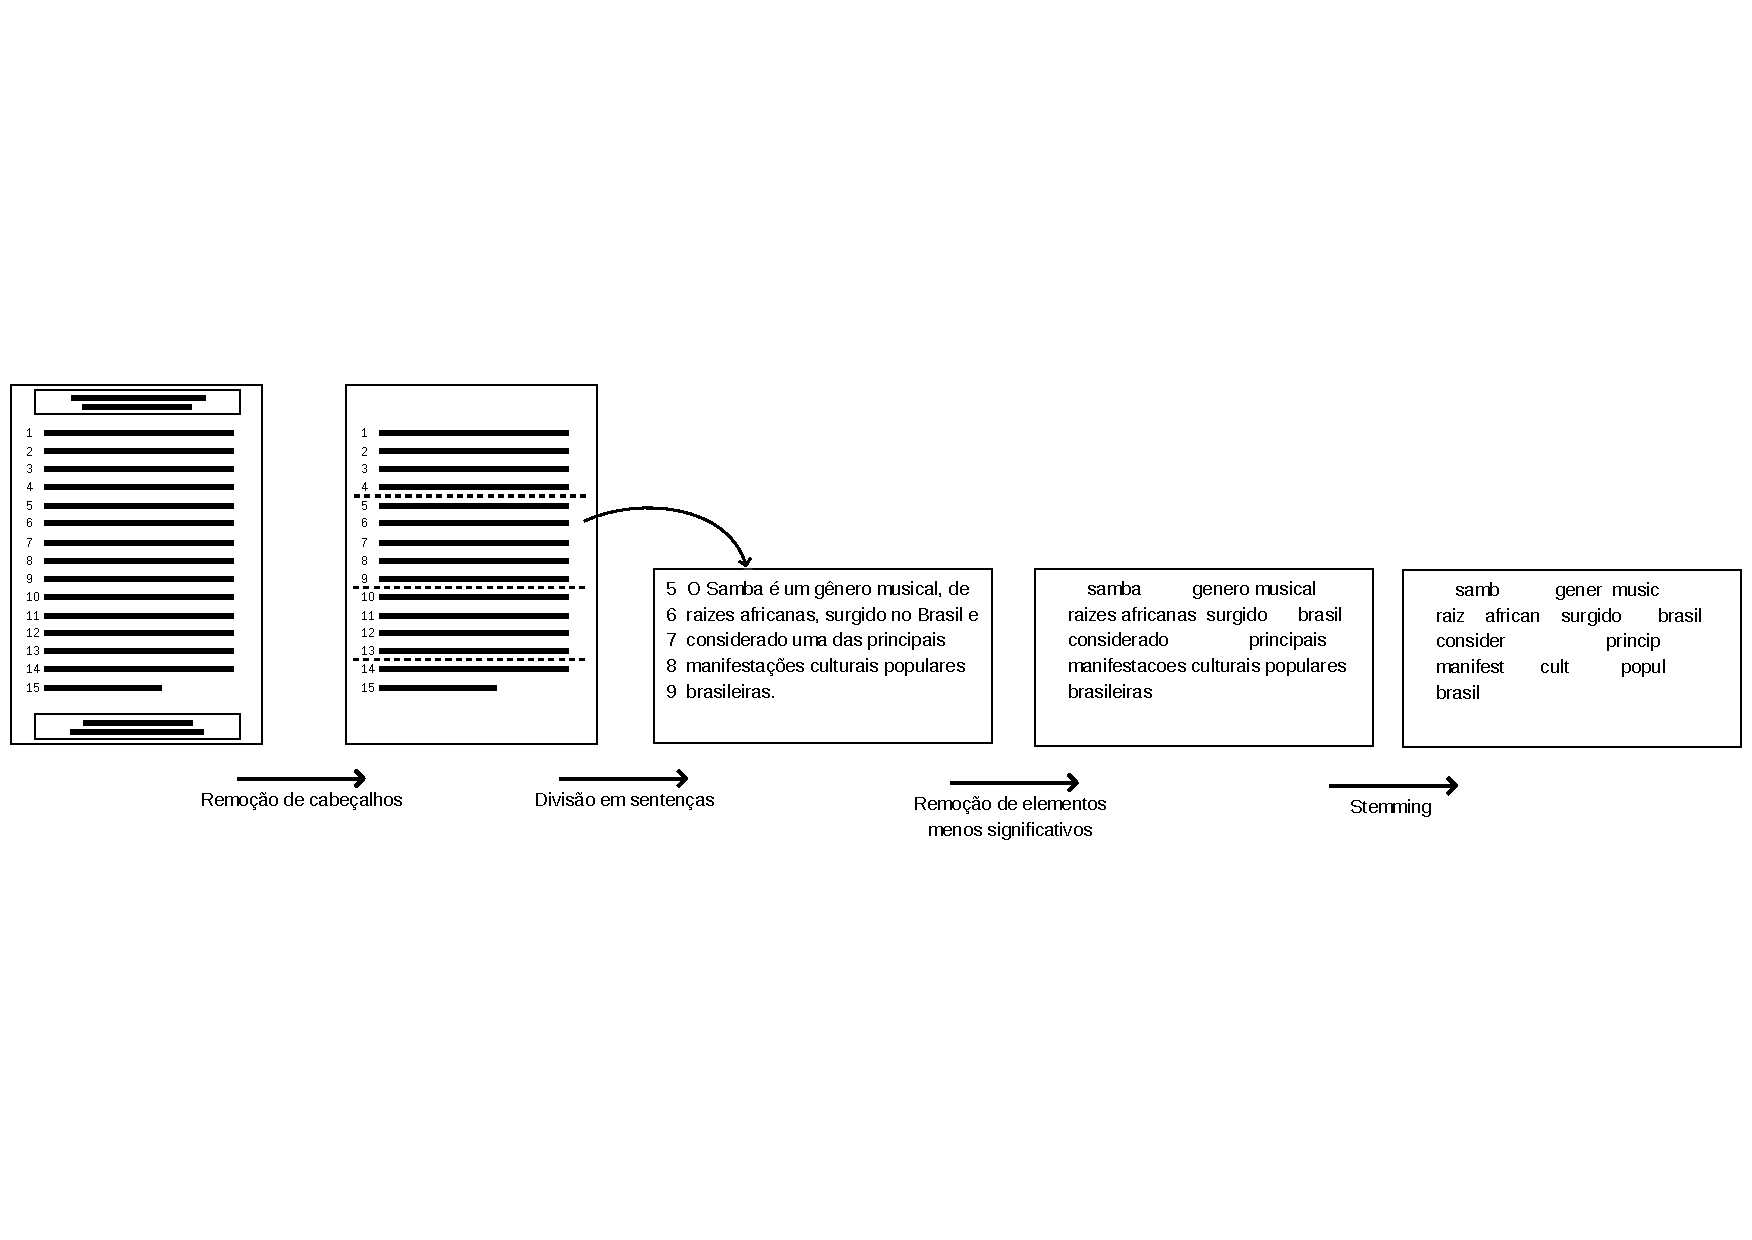
\includegraphics[trim={ 0 180 0 180 },clip,page=1,width=\textwidth]{conteudo/capitulos/figs/pre-process.pdf}

	\caption{Etapa de pré-processamento de um documento que inclui da remoção de elementos menos significativos e a identificação de sentenças}
	\label{fig:preprocessamento-segmentacao}
	\end{figure}
\end{center}



\begin{enumerate}

%  Cabeçalhos e rodapés
\item Remoção de cabeçalhos: as atas contém trechos que podem ser considerados pouco informativos e descartados durante o pré-processamento, como cabeçalhos e rodapés que se misturam aos tópicos tratados na reunião, podendo ser inseridos no meio de um tópico prejudicando tanto os algoritmos de MT e RI, quanto a leitura do texto pelo usuário. Um cabeçalho é a porção de texto que inicia cada página do documento e, de forma semelhante, um rodapé e a porção que as encerra. Detecta-se os cabeçalhos e os rodapés sempre que há uma repetição das primeiras e últimas palavras do documento.


%  Identificação de sentenças
\item Identificação sentenças: Nesse trabalho considera-se as sentenças as menor unidade de informação a ser processada pelos algoritmos de segmentação, por tanto, devem ser identificadas. Ao considerar intuitivamente que uma sentença seja uma sequência de palavras entre sinais de pontuação como ``.'', ``!'' e ``?'', alguns erros poderiam ocorrer quando esses tiverem outra função dentro do texto como em abreviações\footnote{As abreviações são identificadas por meio de uma lista com 234 abreviações conhecidas.}, endereços de internet e datas. Outro problema seriam frases curtas com poucas palavras e que não expressam um conceito completo, mas parte dele. Devido ao estilo de pontuação desses documentos, como encerrar sentenças usando um \textit{``;''} e inserção de linhas extras, foram usadas as regras especiais para identificação de finais de sentença. No Algoritmo~\ref{alg:identificacaofinaisdesent} é mostrado como cada \textit{token} é identificado e marcado com final de sentença.%, esse processo é melhor descrito na Subseção~\ref{subsec:indentificacaosentencas}. % Os detalhes sobre essas regras estão disponíveis para consulta em \urlsoftwares.



\begin{algorithm}
	\SetKwInOut{Input}{Entrada}
	\SetKwInOut{Output}{Saída}
	\SetKwBlock{Inicio}{início}{fim}
	\SetKwFor{ParaTodo}{para todo}{}{fim para todo}
	\SetKwIF{Se}{SenaoSe}{Senao}{}{}{senao se}{senao}{fim se}
	\SetKwFor{Para}{}{}{}
%	\SetKwAlgorithm{Algorithm}{Algoritmo}{}

	
	\Input{Texto}
	\Output{Texto com identificações de finais de sentença}
	
	\ParaTodo {token, marcá-lo como final de sentença se:} {	

	Terminar com um \texttt{!}\\
	Terminar com um \texttt{.} e não for uma abreviação\\
	Terminar em \texttt{.?;} e:
		\Para{}{
			For seguido de uma quebra de parágrafo ou tabulação\\
			O próximo \textit{token} iniciar com  \texttt{(\{["'}\\
			O próximo \textit{token} iniciar com letra maiúscula\\
			O penúltimo caracter  for \texttt{)\}]"'}\\
		}
	}
	
	\caption{Identificação de finais de sentença.}
	\label{alg:identificacaofinaisdesent}
\end{algorithm}


% TODO: "Pra que fazer isso?"


%  Remoção de termos
\item Redução de elementos menos significativos: Removeu-se do textos os termos que não contribuem para a etapa de segmentação, 
	as quais são chamadas de \textit{stop words}. Palavras como artigos, preposições, pronomes, verbos de estado\footnote{Apresentam uma situação inativa, onde o verbo não expressa uma alteração, mas apenas uma propriedade ou condição dos envolvidos.}. Trata-se também como \textit{stop words} as palavras de uso muito frequente dentro de um determinado domínio as quais não são capazes de discriminar textos, portanto também não devem fazer parte dos atributos~\cite{Rezende2003}. Para removê-las, as letras foram convertidas em caixa baixa e usou-se uma lista de 438 palavras para identificá-las. Além disso, eliminou-se a acentuação, sinais de pontuação, numerais e todos os termos menores que três caracteres.

%  Stemming
\item \textit{Stemming}: extraiu-se o radical de cada palavra. Para isso, aplicou-se o algoritmo \textit{Orengo} %\footnote{http://www.inf.ufrgs.br/~viviane/rslp/} 
	para remoção de sufixos~\cite{Alvares2005}.

\end{enumerate}
	



% ==================== Segmentação ===================== %


\subsection{Segmentação}

Como já mencionado, uma ata registra a sucessão de assuntos discutidos em uma reunião, porém apresenta-se com poucas quebras de parágrafo e sem marcações de estrutura, como capítulos, seções ou quaisquer indicações sobre o assunto do texto. Portanto, faz-se necessário descobrir quando há uma mudança de assunto no texto da ata. Para essa tarefa, as técnicas de segmentação de texto recebem uma lista de sentenças, da qual considera cada ponto entre duas sentenças como candidato a limite, ou seja, um ponto onde há transição entre assuntos~\cite{Bokaei2015, Bokaei2016, Misra2009, Sakahara2014}.

As técnicas de segmentação aboradas na Subseção~\ref{sec:segmentacao} divdiem o texto de cada ata em trechos que contêm um assunto relativamente independente, aqui chamdaos de sub-documentos. Esses sub-documentos serão processados por um extrator de tópicos que irá extrair descritores e agrupalos por tópicos.







% ==================== O Corpus ===================== %


\subsection{O Corpus}

% Colocar um trecho de uma ata??

% ->------> Seleção das atas
Selecionou-se um conjunto de atas reais coletadas do Departamento de Computação da UFSCar campus Sorocaba. Analisou-se as atas públicas das reuniões do Conselho de Pós-Graduação e Conselho de Graduação desse departamento das quais foram selecionadas seis atas de cada conselho, sendo cinco referentes a reuniões ordinária e uma reunião extraordinária, totalizando doze documentos. Esses documentos foram escolhidos de forma que o conjunto final contenha atas com tamanhos diferentes (entre 1 e 4 páginas), e maior diversidade de conteúdo.
 % contém tabelas e listas


















